\documentclass[12pt]{article}

% Gói cơ bản
\setcounter{secnumdepth}{0}

\usepackage{graphicx}
\usepackage{float}

\usepackage{url}
\usepackage{pgffor}
\usepackage{array}
\usepackage{geometry}
\geometry{a4paper, margin=1in}
\usepackage{longtable}
\usepackage{tikz}
\usetikzlibrary{calc}
\usepackage{amsmath}
\usepackage{setspace}


% Hỗ trợ tiếng Việt
\usepackage[T5]{fontenc}
\usepackage[utf8]{inputenc}
\usepackage[vietnamese]{babel}

% Hyperlink cho URL
\usepackage[colorlinks=true, linkcolor=blue, urlcolor=blue]{hyperref}

% =========================
% Bìa
% =========================
\geometry{
    top=1.8cm,
    bottom=1.8cm,
    left=2cm,
    right=2cm
}

\setstretch{1.05} % thu nhỏ khoảng cách dòng

\begin{document}
\thispagestyle{empty}

% ===== Khung viền màu xanh cho bìa=====
\begin{tikzpicture}[remember picture, overlay]
    \draw[line width=2pt, blue]
        ($(current page.north west)+(1cm,-1cm)$)
        rectangle
        ($(current page.south east)+(-1cm,1cm)$);
\end{tikzpicture}

% ===== Nội dung bìa=====
\begin{center}
    \vspace*{0.3cm}

    {\Large \bfseries ĐẠI HỌC QUỐC GIA TP.HCM}\\[-2pt]
    {\Large \bfseries TRƯỜNG ĐẠI HỌC CÔNG NGHỆ THÔNG TIN}\\[1.0cm]

    % ===== Logo =====
    \includegraphics[width=5.5cm]{logo.jpg}\\[1.0cm]

    {\Large \bfseries BÁO CÁO ĐỒ ÁN MÔN HỌC}\\[0.2cm]
    {\large \bfseries Kỹ năng nghề nghiệp}\\[0.5cm]
    {\Large \bfseries TUẦN 1}\\[1.2cm]
\end{center}

\noindent
{\bfseries Môn học:} Kỹ năng nghề nghiệp – SS004.Q12 \\[4pt]

{\bfseries Giảng viên hướng dẫn:} Nguyễn Văn Toàn \\[8pt]

{\bfseries Thực hiện bởi sinh viên:}\\[-4pt]

\begin{itemize}
    \setlength{\itemsep}{0pt}
    \setlength{\topsep}{0pt}
    \setlength{\partopsep}{0pt} % giảm spacing giữa các mục
    \item Man Mỹ Phương — MSSV: 24521414
    \item Trần Thu Phương — MSSV: 24521419
    \item Thành Công Vinh — MSSV: 24522027
    \item Nguyễn Văn Vỹ — MSSV: 24522063
    \item Nguyễn Trần Duy Anh — MSSV: 205220393
\end{itemize}

\vspace{0.4cm}

{\bfseries Thời gian thực hiện:} Thứ 6, ngày 28 tháng 11 năm 2025



% =========================
% Lời cảm ơn
% =========================
\newpage
\thispagestyle{empty}
\begin{center}
{\Large \textbf{LỜI CẢM ƠN}}
\end{center}

Lời đầu tiên, em xin gửi lời cảm ơn chân thành và sâu sắc đến thầy Nguyễn Văn Toàn – giảng viên môn Kỹ năng nghề nghiệp (SS004.Q12). Nhờ sự hướng dẫn tận tình và những kiến thức bổ ích thầy đã truyền đạt, em đã có thêm nhiều góc nhìn mới và hiểu biết sâu hơn về các kỹ năng cần thiết cho hành trình học tập cũng như định hướng nghề nghiệp trong tương lai.

Trong suốt quá trình học môn này, em luôn nhận được sự hỗ trợ, chỉ dẫn và những góp ý quý báu từ thầy. Những chia sẻ của thầy không chỉ giúp em hoàn thiện kỹ năng chuyên môn và kỹ năng mềm mà còn là nguồn động lực lớn để em cố gắng hơn mỗi ngày. Dù đã nỗ lực hết mình, em nhận thức rằng bản thân vẫn còn nhiều hạn chế và rất mong sẽ tiếp tục nhận được sự chỉ bảo của thầy trong thời gian tới.

Em xin chân thành cảm ơn thầy vì sự tận tâm và nhiệt huyết trong giảng dạy. Cuối cùng, em kính chúc thầy thật nhiều sức khỏe, niềm vui và thành công trong sự nghiệp giáo dục và nghiên cứu.

\begin{flushright}
Thành phố Hồ Chí Minh, tháng 11 năm 2025
\end{flushright}

% =========================
% Nhận xét của giảng viên
% =========================
% =========================
% NHẬN XÉT CỦA GIẢNG VIÊN (ĐÃ SỬA LỖI)
% =========================
\newpage
\begin{center}
{\Large \textbf{NHẬN XÉT CỦA GIẢNG VIÊN}}
\end{center}

\addcontentsline{toc}{section}{NHẬN XÉT CỦA GIẢNG VIÊN}

\vspace{0.5cm} % Khoảng cách từ tiêu đề xuống dòng đầu tiên

% Sử dụng vòng lặp để tạo 18 dòng kẻ chấm thẳng hàng
% Khoảng cách giữa các dòng là 1.0cm giúp trang thoáng và dễ viết
\noindent
\foreach \i in {1,...,18}{
    \makebox[\linewidth]{\dotfill} \\[0.75cm]
}

% =========================
% Mục lục tự động
% =========================
% =========================
% Mục lục tự động
% =========================
\newpage
\thispagestyle{empty} % ẩn số trang

% Cho phép hiển thị section + subsection trong mục lục
\setcounter{tocdepth}{2}

\begin{center}
{\Large \textbf{MỤC LỤC}}
\end{center}

% Lời cảm ơn và nhận xét không đánh số nhưng có trong mục lục
\section*{LỜI CẢM ƠN}
\addcontentsline{toc}{section}{LỜI CẢM ƠN}

\section*{NHẬN XÉT CỦA GIẢNG VIÊN}
\addcontentsline{toc}{section}{NHẬN XÉT CỦA GIẢNG VIÊN}

% Các phần còn lại đánh số bình thường
\section{HỢP ĐỒNG THÀNH LẬP NHÓM}
\subsection{Thời gian thành lập nhóm}
\subsection{Tên nhóm}
\subsection{Thành viên nhóm}
\subsection{Nguyên tắc làm việc nhóm}
\subsection{Không gian trao đổi và giao tiếp}
\subsection{Mục đích thành lập nhóm}
\subsection{Đánh giá công tác làm việc nhóm}



\section{GIỚI THIỆU VÀ HƯỚNG DẪN CHƠI GAME}
\subsection{Lời mở đầu và giới thiệu chung}
\subsection{Cài đặt và thiết lập}
\subsection{Giao diện người dùng (UI) và điều khiển}
\subsection{Cơ chế Gameplay cốt lõi}
\subsection{Hướng dẫn chơi theo tiến trình}
\subsection{Mẹo nâng cao \& những sai lầm cần tránh}
\subsection{Lời kết và lời mời}

\newpage

% =========================
% Hợp đồng thành lập nhóm
% =========================

\begin{center}
{\Large \textbf{HỢP ĐỒNG THÀNH LẬP NHÓM}}\\[6pt]
\end{center}

\noindent \textbf{Thời gian thành lập:} 24-11-2025

\noindent \textbf{Tên nhóm:} 5 chú cá

\section*{Thành viên:}

\begin{longtable}{|c|m{5cm}|c|}
\hline
\textbf{STT} & \textbf{Họ và tên} & \textbf{MSSV} \\
\hline
1 & Man Mỹ Phương & 24521414 \\
\hline
2 & Trần Thu Phương & 24521419 \\
\hline
3 & Thành Công Vinh & 24522027 \\
\hline
4 & Nguyễn Văn Vỹ & 24522063 \\
\hline
5 & Nguyễn Trần Duy Anh & 205220393 \\
\hline
\end{longtable}

\section*{Nguyên tắc làm việc nhóm:}

Điều 1: Ứng xử văn minh, lịch sự và tôn trọng tất cả các thành viên trong nhóm, trên tinh thần bình đẳng và hợp tác.

Điều 2: Tích cực, chủ động trong việc xây dựng và đóng góp ý kiến cho hoạt động của nhóm.

Điều 3: Có tinh thần trách nhiệm cao với các công việc được giao.

Điều 4: Hoàn thành đầy đủ và đúng thời hạn mọi nhiệm vụ đã được phân công theo kế hoạch nhóm.

Điều 5: Giữ tinh thần đoàn kết, sẵn sàng giúp đỡ và hỗ trợ lẫn nhau trong quá trình làm việc.

Điều 6: Luôn đúng giờ trong các buổi học và họp nhóm. Nếu có lý do đi trễ hoặc vắng mặt, cần báo trước cho nhóm.

Điều 7: Khi gặp khó khăn hoặc trở ngại khiến bản thân không thể hoàn thành công việc đúng hạn, thành viên phải báo trước với nhóm ít nhất 3 ngày để cùng tìm hướng giải quyết.

Điều 8: Nếu có bất đồng ý kiến sẽ giải quyết theo nguyên tắc biểu quyết đa số.

Điều 9: không được gây chia rẽ, mất đoàn kết giữa các thành viên trong nhóm.

Điều 10: Phải hoàn thành nhiệm vụ được giao đúng thời hạn mà không có lý do chính đáng.

Điều 11: Đi học hoặc họp nhóm đúng giờ, tham gia các buổi họp nhóm.

Điều 12: Báo trước cho nhóm về việc vắng mặt hoặc không thể hoàn thành công việc đúng thời hạn theo quy định.

\section*{Không gian trao đổi và giao tiếp}

\subsection*{1. Slack}

Slack là một nền tảng giao tiếp và làm việc nhóm chuyên dụng, được sử dụng rộng rãi trong các doanh nghiệp và môi trường giáo dục.

Công cụ này cho phép sinh viên tạo các kênh (channel) riêng biệt cho từng môn học, dự án hoặc chủ đề, giúp việc trao đổi thông tin trở nên có tổ chức và hiệu quả hơn.

Slack hỗ trợ nhắn tin nhanh, gửi tệp, thực hiện cuộc gọi video, gắn thẻ thành viên và lưu trữ lịch sử trò chuyện, tạo điều kiện thuận lợi cho việc theo dõi tiến độ công việc và đảm bảo tính minh bạch trong giao tiếp nội bộ.

Một ưu điểm nổi bật của Slack là khả năng tích hợp linh hoạt với nhiều công cụ khác như Google Drive, Trello, Zoom, giúp việc quản lý và phối hợp trong các dự án nhóm phức tạp trở nên dễ dàng và chuyên nghiệp hơn.

Link: \url{https://app.slack.com/client/T09DLM2RRNX/C0A00H16K9A}

\subsection*{2. Zalo}

Zalo là nền tảng nhắn tin và trao đổi thông tin phổ biến tại Việt Nam, hỗ trợ nhóm làm việc giao tiếp nhanh chóng và thuận tiện. Với khả năng gửi tin nhắn tức thời, chia sẻ tài liệu, hình ảnh, tạo nhóm trò chuyện và thực hiện cuộc gọi, Zalo giúp các thành viên cập nhật tiến độ, phân công nhiệm vụ và trao đổi ý tưởng hiệu quả. Nhờ tính đơn giản, dễ truy cập trên cả điện thoại và máy tính, Zalo trở thành công cụ giao tiếp linh hoạt hỗ trợ quá trình phối hợp khi thực hiện báo cáo nhóm.

Link: \url{https://zalo.me/g/glejxa926}

\subsection*{3. Google meet}
Google Meet là công cụ họp trực tuyến được nhóm sinh viên sử dụng để trao đổi, thảo luận và cập nhật tiến độ khi làm việc nhóm dự án game Tetris. Nhờ Google Meet, các thành viên có thể tổ chức các buổi họp nhanh, chia sẻ màn hình, thảo luận ý tưởng và giải quyết vấn đề cùng nhau, bất kể ở đâu, giúp nâng cao hiệu quả phối hợp và đảm bảo dự án tiến triển suôn sẻ.

Link: \url{https://meet.google.com/hdn-wtzq-fmo}

\subsection*{4. Google Docs (Tài liệu Google)}

Google Docs là một công cụ cộng tác trực tuyến phổ biến, được sử dụng rộng rãi trong môi trường học tập và làm việc nhóm.

Nền tảng này cho phép nhiều người dùng cùng chỉnh sửa tài liệu trong cùng một thời điểm, theo dõi lịch sử thay đổi và đưa ra nhận xét trực tiếp trên nội dung đang làm việc.

Tất cả các chỉnh sửa đều được tự động lưu trữ, giúp hạn chế rủi ro mất dữ liệu.

Ngoài ra, Google Docs còn tích hợp chặt chẽ với các công cụ khác trong hệ sinh thái Google như Google Sheets, Google Slides và Google Drive, cho phép nhóm soạn thảo báo cáo, phân tích số liệu, thiết kế bài thuyết trình và lưu trữ tài liệu chung một cách hiệu quả và thuận tiện.

Link: \href{https://docs.google.com/document/d/1do6Aa7rRsqR6zIB9B6g-Lp9p4E3hvgJRdrln6y5CTVo}{Dàn ý Tetris Game 1}



\subsection*{5. Word}

Công cụ soạn thảo văn bản giúp mỗi cá soạn thảo nội dung được phân công trong phần làm việc nhóm. Dữ liệu của cá nhân được lưu lại ngay trên máy để dễ dàng chỉnh sửa khi mà không cần mạng internet.

\subsection*{6. Overleaf}

Overleaf là một nền tảng soạn thảo LaTeX trực tuyến cho phép nhiều thành viên trong nhóm làm việc đồng thời trên cùng một tài liệu. Môi trường biên dịch tích hợp sẵn giúp hiển thị kết quả theo thời gian thực mà không cần cài đặt thêm phần mềm. Nhờ hỗ trợ cộng tác trực tiếp, quản lý phiên bản tự động và khả năng chia sẻ dễ dàng qua liên kết hoặc email, Overleaf rất phù hợp cho các nhóm thực hiện báo cáo, bài nghiên cứu hay luận văn yêu cầu định dạng LaTeX thống nhất và chính xác.

Link: \url{https://github.com/phun11/Latex-Tetris-Game}

\noindent \url{https://www.overleaf.com/read/brsdkxmtznzz#54f937}

\subsection*{7. Github}

GitHub là nền tảng quản lý mã nguồn sử dụng hệ thống kiểm soát phiên bản Git, cho phép nhóm lưu trữ, theo dõi và đồng bộ hóa toàn bộ tệp dự án trong một kho lưu trữ chung. Nhờ cơ chế commit, branch và pull request, các thành viên có thể làm việc song song mà vẫn đảm bảo kiểm soát được lịch sử thay đổi và tránh xung đột nội dung. GitHub đặc biệt hữu ích khi kết hợp với Overleaf để quản lý nguồn LaTeX, giúp nhóm duy trì cấu trúc tài liệu rõ ràng, minh bạch và dễ dàng phối hợp trong quá trình viết báo cáo.

Link: \url{https://github.com/phun11/Tetris-Game}

\section*{Mục đích thành lập nhóm}

1. Nâng cao kỹ năng làm việc nhóm và các kỹ năng mềm khác cho các thành viên.

2. Hỗ trợ, động viên lẫn nhau để hoàn thành tốt nhiệm vụ và đạt kết quả cao trong môn học.

\section*{VII. Đánh giá công tác làm việc nhóm}

\subsection*{1. Bảng tiêu chí đánh giá}

\begin{longtable}{|m{4cm}|m{3cm}|m{2.5cm}|m{3cm}|m{2.5cm}|}
\hline
\textbf{Tiêu chí đánh giá} & \textbf{Xuất sắc} & \textbf{Tốt} & \textbf{Bình thường} & \textbf{Kém} \\
\hline
1. Thái độ làm việc & Chủ động nhận và hoàn thành tốt nhiệm vụ được giao & Hoàn thành nhiệm vụ được giao đúng yêu cầu & Hoàn thành nhiệm vụ sau khi được nhắc nhở & Không hoàn thành nhiệm vụ được giao \\
\hline
2. Quản lý thời gian & Hoàn thành nhiệm vụ trước hạn hoặc đúng hạn theo lịch phân công & Hoàn thành nhiệm vụ đúng hạn hoặc trễ không quá 12 giờ theo lịch phân công & Hoàn thành nhiệm vụ trễ nhưng không quá 24 giờ theo lịch phân công & Không hoàn thành nhiệm vụ hoặc trễ quá 24 giờ theo lịch phân công \\
\hline
3. Nghiên cứu tài liệu & Chủ động tìm kiếm, tổng hợp và chia sẻ tài liệu hữu ích cho nhóm & Tìm kiếm tài liệu phục vụ phần việc được giao & Có nghiên cứu nhưng chưa đầy đủ, cần hỗ trợ thêm & Không tìm hiểu hoặc không đóng góp tài liệu cho nhóm \\
\hline
4. Phối hợp làm việc nhóm & Chủ động hỗ trợ, hợp tác tốt với các thành viên khác & Phối hợp tốt trong phạm vi công việc được giao & Chỉ hợp tác khi được yêu cầu & Thiếu tinh thần hợp tác, làm việc tách biệt \\
\hline
5. Giải quyết vấn đề được giao & Chủ động tìm kiếm giải pháp, đề xuất hướng xử lý hiệu quả & Tìm kiếm giải pháp phù hợp theo phân công & Tham gia góp ý nhưng chưa tìm ra hướng giải quyết cụ thể & Không tham gia giải quyết vấn đề \\
\hline
6. Kết nối, giao tiếp hiệu quả & Chủ động liên lạc, trao đổi thường xuyên, rõ ràng với nhóm & Luôn giữ liên lạc và phản hồi kịp thời & Thỉnh thoảng phản hồi chậm hoặc mất liên lạc trong 24 giờ & Không liên lạc, không phản hồi \\
\hline
7. Đóng góp ý kiến & Chủ động đưa ra ý kiến, sáng kiến giúp cải thiện chất lượng công việc & Đưa ra ý kiến khi liên quan đến phần việc cá nhân & Chỉ phát biểu khi được yêu cầu & Không tham gia đóng góp ý kiến \\
\hline
8. Hoàn thành công việc đúng hạn & Hoàn thành công việc vượt mong đợi, chất lượng cao & Hoàn thành công việc đúng hạn, đạt yêu cầu & Hoàn thành công việc trễ nhưng đảm bảo chất lượng & Không hoàn thành công việc đúng thời hạn hoặc không đạt yêu cầu \\
\hline
\end{longtable}

\subsection*{2. Cam kết nhóm}

Tất cả thành viên trong nhóm cam kết hợp tác với nhau trên tinh thần vui vẻ, tôn trọng và hết mình hỗ trợ lẫn nhau.

Các thành viên không vi phạm điều lệ nhóm, hoàn thành tốt nhiệm vụ cá nhân và đóng góp tích cực cho mục tiêu chung mà nhóm đã đề ra.

Thành viên nhóm đã đọc, hiểu và đồng ý với các điều khoản, hướng dẫn được nêu trong hợp đồng này.

Hợp đồng lập nhóm đã được thông qua và ký kết.

\vspace{1cm}

\noindent Thành phố Hồ Chí Minh, ngày 28 tháng 11 năm 2025

\vspace{1.5cm}


% Dòng chữ nằm bên phải + tăng 2 size
\begin{flushright}
    {\Large \textit{Các thành viên ký tên:}}
\end{flushright}

\vspace{0.7cm}

% Chữ ký chia thành 2 hàng, mỗi hàng 2 người
\begin{center}
\begin{tabular}{ccc}
    \includegraphics[width=4cm]{mphun.jpg} &
    \includegraphics[width=4cm]{duyanh.jpg} &
    \includegraphics[width=4cm]{congvinh.jpg} \\
    [1.2cm]
    \includegraphics[width=4cm]{thuphun.jpg} &
    \includegraphics[width=4cm]{vy.jpg} &
    {}
\end{tabular}
\end{center}


\vspace{3cm}
\newpage

\section*{B. GIỚI THIỆU VÀ HƯỚNG DẪN CHƠI GAME}

\section*{I. Lời mở đầu và giới thiệu chung}

Chào mừng bạn đến với phiên bản Tetris của chúng tôi!

Tetris là trò chơi xếp khối kinh điển, được yêu thích trên toàn thế giới. Đặc biệt, trò chơi này phù hợp với mọi lứa tuổi bởi nó không những mang lại sự thư giãn, giải trí sau những giờ học hoặc làm việc căng thẳng mà còn thách thức tư duy, cải thiện sự tập trung, trí nhớ và rèn luyện phản xạ, tư duy chiến lược.

Tetris là một trò chơi điện tử giải đố kinh điển, phổ biến nhất mọi thời đại được phát triển bởi Alexey Pajitnov, một kỹ sư phần mềm người Liên Xô. Tên "Tetris" là sự kết hợp của "tetra" (nghĩa là số bốn trong tiếng Hy Lạp) và "tennis" (môn thể thao yêu thích của tác giả).

Trong lối chơi Tetris điển hình, các hình khối tetromino đầy màu sắc rơi từ trên xuống, nhiệm vụ của bạn là phải sắp xếp chúng thành một chồng. Khi một hàng hoặc cột của bảng trò chơi được lấp đầy, nó sẽ biến mất và điểm số của bạn sẽ tăng lên.

Phiên bản của chúng tôi sở hữu lối chơi gần giống bản cổ điển nhưng mang đến trải nghiệm mượt mà, hiện đại, đồng thời còn bổ sung một số tính năng mới như Next Queue và lưu điểm cao nhất.

\section*{II. Cài đặt và thiết lập}

\subsection*{1. Cài đặt}

Quy trình cài đặt gồm 3 bước đơn giản:

\begin{itemize}
    \item \textbf{Bước 1: Truy cập và Tải về.} Truy cập vào đường dẫn GitHub của dự án. Tại giao diện chính, tìm và chọn tải xuống tệp nén của trò chơi.
    Link: https://github.com/phun11/Tetris-Game
    \item \textbf{Bước 2: Giải nén.} Sau khi tải xong, nhấp chuột phải vào tệp tin vừa tải về và giải nén toàn bộ thư mục trò chơi.
    \item \textbf{Bước 3: Mở game.} Truy cập vào thư mục vừa giải nén, tìm file thực thi của trò chơi và nhấp đúp chuột để bắt đầu chơi.
\end{itemize}

\subsection*{2. Tối ưu}

Sau khi mở game, để có trải nghiệm chơi mượt mà và tập trung nhất, bạn nên kiểm tra nhanh các thiết lập:

\begin{itemize}
    \item \textbf{Đồ họa \& Hiển thị:} Trò chơi mặc định chạy ở chế độ cửa sổ tiêu chuẩn. Đảm bảo độ phân giải màn hình của bạn phù hợp để nhìn rõ các khối gạch và điểm số.
    \item \textbf{Âm thanh:} Kiểm tra loa hoặc tai nghe để tận hưởng nhạc nền và hiệu ứng âm thanh (SFX) khi xếp gạch. Bạn có thể điều chỉnh âm lượng hệ thống sao cho vừa đủ nghe, giúp tăng sự tập trung.
\end{itemize}

\section*{III. Giao diện người dùng (UI) và điều khiển}

\subsection*{1. Khu vực Playfield (15 × 20)}

Đây là không gian chính của trò chơi, có kích thước tiêu chuẩn:

Chiều rộng: 15 ô

Chiều cao: 20 ô

Tại đây, các khối Tetrimino rơi từ trên xuống. Nhiệm vụ của bạn là sắp xếp các khối sao cho chúng tạo thành các hàng đầy, từ đó xóa hàng và ghi điểm. Người chơi cần quan sát, dự đoán vị trí rơi của các khối và xoay hoặc di chuyển chúng để xếp chồng một cách hợp lý, tránh để khối chồng đầy Playfield dẫn tới kết thúc trò chơi.

\subsection*{2. Khu vực Next Queue (Khối tiếp theo)}

Nằm ở góc phải màn hình, đây là vùng hiển thị khối Tetrimino sẽ xuất hiện tiếp theo. Khu vực này giúp người chơi xem trước để lên chiến lược hợp lý. Bạn nên quan sát Next Queue thường xuyên để tối ưu hóa việc xếp khối, giảm sai sót và tăng khả năng đạt điểm cao.

\subsection*{3. Điểm số (Score)}

Điểm số được hiển thị rõ ràng trên giao diện, ở cạnh Playfield, giúp người chơi theo dõi thành tích của mình.

Điểm tăng mỗi khi bạn xoá hàng. Xoá càng nhiều hàng cùng lúc, điểm càng cao.

\subsection*{4. Level hiện tại (Level)}

Level thể hiện độ khó của ván chơi. Khi bạn clear mỗi 10 hàng, level sẽ tăng, tốc độ các khối rơi cũng tăng lên 10\%.

Hệ thống level giúp trò chơi ngày càng có tính thử thách, không gây nhàm chán, giúp bạn rèn luyện phản xạ nhanh và tư duy chiến lược.

\subsection*{5. Hệ thống điều khiển}

Bạn có thể điều khiển khối Tetrimino bằng các phím sau:

Phím A/D: di chuyển khối Tetrimino sang trái/phải

Phím W: xoay khối Tetrimino theo chiều kim đồng hồ.

Phím S: tăng tốc rơi (soft drop).

Phím X: thả nhanh (hard drop).

Lưu ý: luôn lưu/high score tự động hoặc theo file nếu game hỗ trợ.

\section*{IV. Cơ chế Gameplay cốt lõi}

\subsection*{1. Các loại khối}

Các Tetromino: I, O, T, S, Z, J, L.

\noindent{Hình ảnh minh họa :}

\begin{center}
    \includegraphics[width=0.9\textwidth]{hinhanhvythe.jpg}
\end{center}
\renewcommand{\arraystretch}{2.0} % chỉnh hệ số giãn dòng
\begin{tabular}{|c|c|>{\centering\arraybackslash}p{8cm}|}
\hline
\textbf{Khối} & \textbf{Tên} & \textbf{Đặc điểm} \\
\hline
I & I-Tetrimino & Dài 4 ô thẳng hàng. Mạnh trong việc tạo Tetris (xóa 4 dòng). \\
\hline
O & O-Tetrimino & Hình vuông 2×2, không thay đổi hình dạng khi xoay. \\
\hline
T & T-Tetrimino & Dạng chữ T, linh hoạt, dễ xoay và xử lý nhiều tình huống. \\
\hline
J & J-Tetrimino & Hình chữ L ngược, tạo rãnh tốt. \\
\hline
L & L-Tetrimino & Hình chữ L, dùng để lấp góc hiệu quả. \\
\hline
S & S-Tetrimino & Dạng ziczac, thường khó xử lý nếu stack không phẳng. \\
\hline
Z & Z-Tetrimino & Tương tự S nhưng đối xứng ngược. \\
\hline
\end{tabular}

\vspace{1em}

\subsection*{1.2. Mỗi khối có hình dạng và cách xoay khác nhau.}
\begin{itemize}
    \item \textbf{Nguyên tắc xoay tổng  :}


Mỗi Tetromino có 4 trạng thái xoay tương ứng với các góc:
\[
0^\circ \rightarrow 90^\circ \rightarrow 180^\circ \rightarrow 270^\circ \rightarrow 0^\circ
\]

\item \textbf {Khi người chơi nhấn phím xoay, trò chơi thực hiện các bước:}

Khi bạn nhấn phím xoay, trò chơi sẽ lấy hình dạng và vị trí hiện tại của Tetrimino để chuẩn bị cho thao tác xoay. Đây là bước quan trọng để hệ thống biết khối nào đang được thao tác.

\vspace{0.03cm}
Tiếp theo, khối sẽ được xoay 90° theo chiều kim đồng hồ. Việc này thay đổi hướng và hình dạng của Tetrimino, giúp bạn linh hoạt sắp xếp các khối để lấp đầy các khoảng trống trên bảng chơi.

\vspace{0.03cm}
Ngay sau khi xoay, trò chơi sẽ kiểm tra xem khối có va chạm hay không. Khối không được vượt ra ngoài biên trái/phải, không rơi xuống sàn và không chồng lên các khối đã cố định. Việc kiểm tra này đảm bảo Tetrimino luôn nằm đúng vị trí và trò chơi diễn ra mượt mà.

\vspace{0.03cm}
Nếu xảy ra va chạm, cơ chế wall kick sẽ được kích hoạt. Trò chơi sẽ tự động đẩy khối sang trái hoặc phải 1–2 ô để tìm vị trí hợp lệ. Nhờ vậy, Tetrimino vẫn có thể xoay ngay cả khi gần tường hoặc sát các khối cố định, hạn chế tình trạng kẹt khối.

\vspace{0.03cm}
Trong trường hợp khối vẫn không thể đặt vào vị trí hợp lệ sau khi thử wall kick, thao tác xoay sẽ bị hủy và Tetrimino giữ nguyên trạng thái ban đầu. Điều này giúp trò chơi luôn ổn định và bạn không mất kiểm soát khối.

\vspace{0.03cm}
Nhờ cơ chế xoay kết hợp kiểm tra va chạm và wall kick, việc xoay Tetrimino trở nên mượt mà, dễ điều khiển và hạn chế tình trạng kẹt sát tường, mang lại trải nghiệm chơi Tetris trơn tru và thú vị hơn.

\vspace{0.03cm}
Nhờ cơ chế xoay + kiểm tra va chạm + wall kick, việc điều khiển Tetromino trở nên mượt mà và ổn định.
\end{itemize}
%---------------------------------------------------------------

\subsection*{2. Hệ thống điểm \& xếp hạng}

\begin{itemize}
    \item \textbf{Tính điểm}
\end{itemize}

Trong trò chơi, người chơi được thưởng điểm dựa trên số lượng hàng bị xóa trong một lượt.  
Xóa càng nhiều hàng thì điểm càng cao:

\begin{itemize}
    \item[\text{\large$\circ$}] 1 dòng xóa = \textbf{40 điểm}
    \item[\text{\large$\circ$}] 2 dòng xóa = \textbf{100 điểm}
    \item[\text{\large$\circ$}] 3 dòng xóa = \textbf{300 điểm}
    \item[\text{\large$\circ$}] 4 dòng xóa (Tetris) = \textbf{1200 điểm}
\end{itemize}
\begin{itemize}
    \item \textbf{Next Queue:} hiển thị trước khối tiếp theo, giúp người chơi chủ động lên chiến lược.  
\end{itemize}

\begin{itemize}
    \item \textbf{Tăng tốc độ rơi:}  sau mỗi 10 dòng được xóa, tốc độ rơi của khối tăng 10\%, khiến trò chơi thách thức dần theo thời gian.
\end{itemize}

% --------------------------------------------------------------

\subsection*{3. Khi nào trò chơi kết thúc?}

Trò chơi sẽ kết thúc khi không còn không gian để tạo vị trí xuất hiện cho khối mới.

\begin{itemize}
    \item Gạch chạm đỉnh → không thể sinh khối mới → \textbf{Game Over}
    \item Màn hình hiển thị: tổng điểm, số hàng đã xóa và level đạt được.
\end{itemize}


\section*{V. Hướng dẫn chơi theo tiến trình}

\subsection*{1. Bắt đầu}

Khi mở game, bạn sẽ thấy giao diện tuỳ chọn các chế độ phổ biến bao gồm:

\begin{itemize}
    \item \textbf{Marathon}: chơi đến khi thua, mục tiêu đạt mức điểm nhất định.
    \item \textbf{Sprint / 40 Lines}: hoàn thành 40 hàng nhanh nhất.
    \item \textbf{Ultra}: ghi điểm trong 2 phút.
    \item \textbf{Endless}: chơi vô hạn đến khi thua.
\end{itemize}

Sau khi chọn chế độ, bạn sẽ cần chọn độ khó (level càng cao, tốc độ rơi gạch càng nhanh). Có 3 mức độ:

\begin{itemize}
    \item Easy
    \item Medium
    \item Hard
\end{itemize}

\textbf{Khuyến nghị cho người mới:} nên bắt đầu với chế độ \textbf{Marathon} hoặc \textbf{Endless} ở mức \textbf{Easy} để làm quen tốc độ và điều khiển.

\subsection*{2. Chơi game}

Mục tiêu chính của trò chơi là xếp các khối để tạo thành một hoặc nhiều hàng hoàn chỉnh. Khi lấp đầy hàng, chúng sẽ biến mất và người chơi nhận điểm dựa trên số hàng xoá liên tiếp và tốc độ chơi.

\medskip

Theo dõi khu vực \textbf{Next Queue} (hiển thị khối sẽ xuất hiện tiếp theo, nằm bên phải màn hình) để lập kế hoạch sắp xếp. Điều này giúp chuẩn bị vị trí cho các khối dài để tạo \textbf{Tetris} (xoá 4 hàng cùng lúc).

\medskip

\noindent \textbf{Các điều khiển quan trọng:}

\begin{itemize}
    \item \textbf{Phím A/D}: di chuyển khối sang trái / phải.
    \item \textbf{Phím W}: xoay khối theo chiều kim đồng hồ.
    \item \textbf{Phím S (Soft Drop)}: tăng tốc độ rơi nhưng vẫn điều khiển được.
    \item \textbf{Phím X (Hard Drop)}: thả khối xuống đáy ngay lập tức, ghi thêm điểm.
\end{itemize}

\textit{Lưu ý:} Người mới nên dùng Soft Drop để dễ kiểm soát; khi quen hãy dùng Hard Drop để tăng tốc độ chơi và ghi điểm.

\medskip

\noindent \textbf{Cách ghi điểm:}

\begin{itemize}
    \item Clear 1 line → điểm thấp.
    \item Clear 2 lines → điểm cao hơn.
    \item Clear 3 lines → nhiều điểm hơn nữa.
    \item Clear 4 lines (\textbf{Tetris}) → điểm rất cao.
    \item Combo liên tục → \textit{bonus points}.
    \item Hard drop / Soft drop → nhận thêm điểm cho mỗi khối.
\end{itemize}

\textbf{Lưu ý quan trọng:} Trò chơi sẽ \textbf{tăng level} sau mỗi số hàng nhất định (thường 10). Level càng cao, gạch rơi càng nhanh. Người mới nên giữ stack thấp để tránh áp lực khi tốc độ tăng.

\subsection*{3. Kết thúc trò chơi}

Trò chơi kết thúc khi:

\begin{itemize}
    \item gạch chạm đỉnh,
    \item hết thời gian,
    \item hoàn thành số hàng quy định (tuỳ chế độ).
\end{itemize}

Màn hình kết thúc hiển thị:

\begin{itemize}
    \item Tổng điểm
    \item Thời gian (tính đến mili giây)
    \item Cấp độ đã đạt được
    \item Tổng số hàng đã xoá
    \item Combo cao nhất
\end{itemize}

Các lựa chọn sau khi kết thúc:

\begin{itemize}
    \item Restart (chơi lại)
    \item Lưu và cập nhật điểm (kỷ lục)
    \item Xem bảng xếp hạng
\end{itemize}

\section*{VI. Mẹo nâng cao \& những sai lầm cần tránh }

\begin{itemize}
    \item[-] {Hạn chế tạo khe trống, đặc biệt ở gần đáy}
\end{itemize}

Bạn nên tránh tạo ra các khe trống, đặc biệt là ở khu vực gần đáy.  
Những khoảng hở này thường rất khó lấp đầy và dễ khiến các khối phía trên bị dồn lên cao, làm tăng nguy cơ thua cuộc.

\begin{itemize}
    \item[-] {Tạo combo xóa nhiều hàng cùng lúc để ghi điểm cao}
\end{itemize}

Việc xóa nhiều hàng liên tiếp hoặc xóa nhiều hàng trong một lần sẽ giúp tăng điểm đáng kể.  
Vì vậy, người chơi nên xây dựng chiến thuật đặt khối hợp lý để tạo ra combo, tối ưu hóa số điểm qua từng lượt.

\begin{itemize}
     \item[-] {Ưu tiên sinh tồn khi tốc độ tăng, không quá mạo hiểm đặt khối}
\end{itemize}

Khi tốc độ rơi của các khối ngày càng nhanh, người chơi nên tập trung vào việc giữ playfield ổn định.  
Đừng quá mạo hiểm đặt các khối khó chỉ để kiếm thêm điểm, vì một sai sót nhỏ có thể khiến bàn chơi bị đầy rất nhanh.

\begin{itemize}
    \item[-] {Lưu ý: luôn sao lưu High Score nếu game có tính năng này}
\end{itemize}

Nếu trò chơi hỗ trợ tính năng lưu High Score, người chơi nên thường xuyên kiểm tra hoặc sao lưu để tránh mất dữ liệu thành tích.  
Điều này giúp bạn theo dõi tiến bộ và đặt ra mục tiêu rõ ràng hơn cho các lần chơi sau.

\section*{VII. Lời kết và lời mời}

Tetris không chỉ là trò chơi giải trí, mà còn là bài tập rèn luyện trí não, giúp bạn thư giãn sau những giờ học tập hay làm việc căng thẳng.

Hãy tải game và bước vào hành trình xếp khối đầy thử thách! Chinh phục từng khối, phá vỡ kỷ lục của chính bạn và trở thành bậc thầy Tetris.

\section{Cơ sở lý thuyết và phân tích thuật toán trong game}

\subsection{I. Các kỹ năng và thuật toán nhóm đã sử dụng}

\subsubsection{1. Kỹ năng lập trình C++ cơ bản và nâng cao}

Nhóm đã vận dụng các kỹ năng lập trình C++ như:
\begin{itemize}
    \item Sử dụng mảng 2 chiều để quản lý bàn chơi (board[H][W]) và hình dạng khối (blocks[7][4][4]).
    \item Sử dụng con trỏ và cấp phát động (new, delete) để quản lý các khối Tetris trong quá trình chơi.
    \item Tổ chức chương trình theo hàm nhằm tách biệt các chức năng: vẽ giao diện, xử lý va chạm, xóa dòng, cập nhật điểm số,…
\end{itemize}

\subsubsection{2. Lập trình hướng đối tượng (OOP)}

Game Tetris được xây dựng dựa trên mô hình lập trình hướng đối tượng, cụ thể:
\begin{itemize}
    \item \textbf{Lớp Piece (lớp cơ sở)}
    \begin{itemize}
        \item Đại diện cho một khối Tetris bất kỳ.
        \item Chứa dữ liệu hình dạng (shape[4][4]) và các phương thức chung:
        \begin{itemize}
            \item rotate() : xoay khối
            \item getCell() : lấy giá trị từng ô
        \end{itemize}
        \item Sử dụng hàm ảo (virtual function) để cho phép đa hình khi xoay khối.
    \end{itemize}

    \item \textbf{Các lớp dẫn xuất (IPiece, OPiece, TPiece, SPiece, ZPiece, JPiece, LPiece)}
    \begin{itemize}
        \item Kế thừa từ lớp Piece.
        \item Áp dụng kế thừa (inheritance) để tái sử dụng mã nguồn.
        \item Riêng OPiece ghi đè (override) hàm rotate() để đảm bảo khối O không xoay.
    \end{itemize}

    \item \textbf{Đa hình (Polymorphism)}
    \begin{itemize}
        \item Con trỏ Piece* được sử dụng để quản lý các khối khác nhau một cách thống nhất.
        \item Việc gọi rotate() được quyết định động theo từng loại khối.
    \end{itemize}

    \item \textbf{Hàm Factory (createPiece)}
    \begin{itemize}
        \item Áp dụng mô hình Factory Pattern để sinh khối Tetris ngẫu nhiên dựa trên loại khối.
    \end{itemize}
\end{itemize}

\subsubsection{3. Thuật toán xoay khối (Rotation Algorithm)}

Nhóm sử dụng thuật toán xoay ma trận 4×4 theo chiều kim đồng hồ:
\begin{verbatim}
temp[j][3 - i] = shape[i][j]
\end{verbatim}

Thuật toán này cho phép:
\begin{itemize}
    \item Xoay khối 90 độ
    \item Áp dụng chung cho mọi khối (trừ khối O)
\end{itemize}

\subsubsection{4. Thuật toán kiểm tra va chạm (Collision Detection)}

\begin{itemize}
    \item Kiểm tra khối có thể di chuyển hay không bằng cách:
    \begin{itemize}
        \item So sánh vị trí tiếp theo với biên trái, biên phải, đáy bàn chơi
        \item Kiểm tra va chạm với các khối đã cố định trên board
    \end{itemize}
    \item Được triển khai trong hàm canMove(dx, dy).
\end{itemize}

\subsubsection{5. Thuật toán xóa dòng (Line Clearing Algorithm)}

\begin{itemize}
    \item Duyệt từ dưới lên trên bàn chơi.
    \item Kiểm tra dòng có đầy đủ ô hay không.
    \item Khi xóa dòng:
    \begin{itemize}
        \item Dịch toàn bộ các dòng phía trên xuống 1 đơn vị.
    \end{itemize}
    \item Thuật toán đảm bảo:
    \begin{itemize}
        \item Có thể xóa nhiều dòng liên tiếp.
        \item Phù hợp với luật Tetris chuẩn.
    \end{itemize}
\end{itemize}

\subsubsection{6. Thuật toán tính điểm và cấp độ}

\begin{itemize}
    \item Tính điểm theo số dòng xóa cùng lúc:
    \begin{itemize}
        \item 1 dòng: 40 điểm
        \item 2 dòng: 100 điểm
        \item 3 dòng: 300 điểm
        \item 4 dòng: 1200 điểm
    \end{itemize}
    \item Cấp độ (Level) tăng theo tổng số dòng đã xóa.
    \item Tốc độ rơi được tăng dần theo level bằng cách giảm thời gian Sleep().
\end{itemize}

\subsubsection{7. Quản lý thời gian và chế độ chơi}

\begin{itemize}
    \item Sử dụng GetTickCount() để đo thời gian thực.
    \item Cài đặt nhiều chế độ chơi:
    \begin{itemize}
        \item Marathon: chơi đến khi thua
        \item Sprint: kết thúc khi xóa đủ 40 dòng
        \item Ultra: tính điểm trong 120 giây
    \end{itemize}
    \item Áp dụng điều kiện kết thúc khác nhau cho từng chế độ.
\end{itemize}

\subsubsection{8. Thư viện và công cụ sử dụng}

\begin{itemize}
    \item \textless iostream\textgreater : nhập xuất dữ liệu
    \item \textless conio.h\textgreater : bắt phím không cần Enter (\_getch, \_kbhit)
    \item \textless windows.h\textgreater :
    \begin{itemize}
        \item Điều khiển con trỏ (gotoxy)
        \item Ẩn con trỏ console
        \item Tô màu ký tự
        \item Quản lý thời gian và tốc độ (Sleep, GetTickCount)
    \end{itemize}
    \item Sử dụng Console API của Windows để xây dựng giao diện text-based.
\end{itemize}

\subsubsection{9. Kỹ năng thiết kế game}

\begin{itemize}
    \item Tổ chức vòng lặp game (Game Loop) rõ ràng:
    \begin{itemize}
        \item Nhận input
        \item Cập nhật logic
        \item Render giao diện
    \end{itemize}
    \item Phân tách logic xử lý và hiển thị.
    \item Quản lý tài nguyên động, tránh rò rỉ bộ nhớ.
\end{itemize}

\subsection{II. Sơ đồ diagram}

\begin{figure}[H]
    \centering
    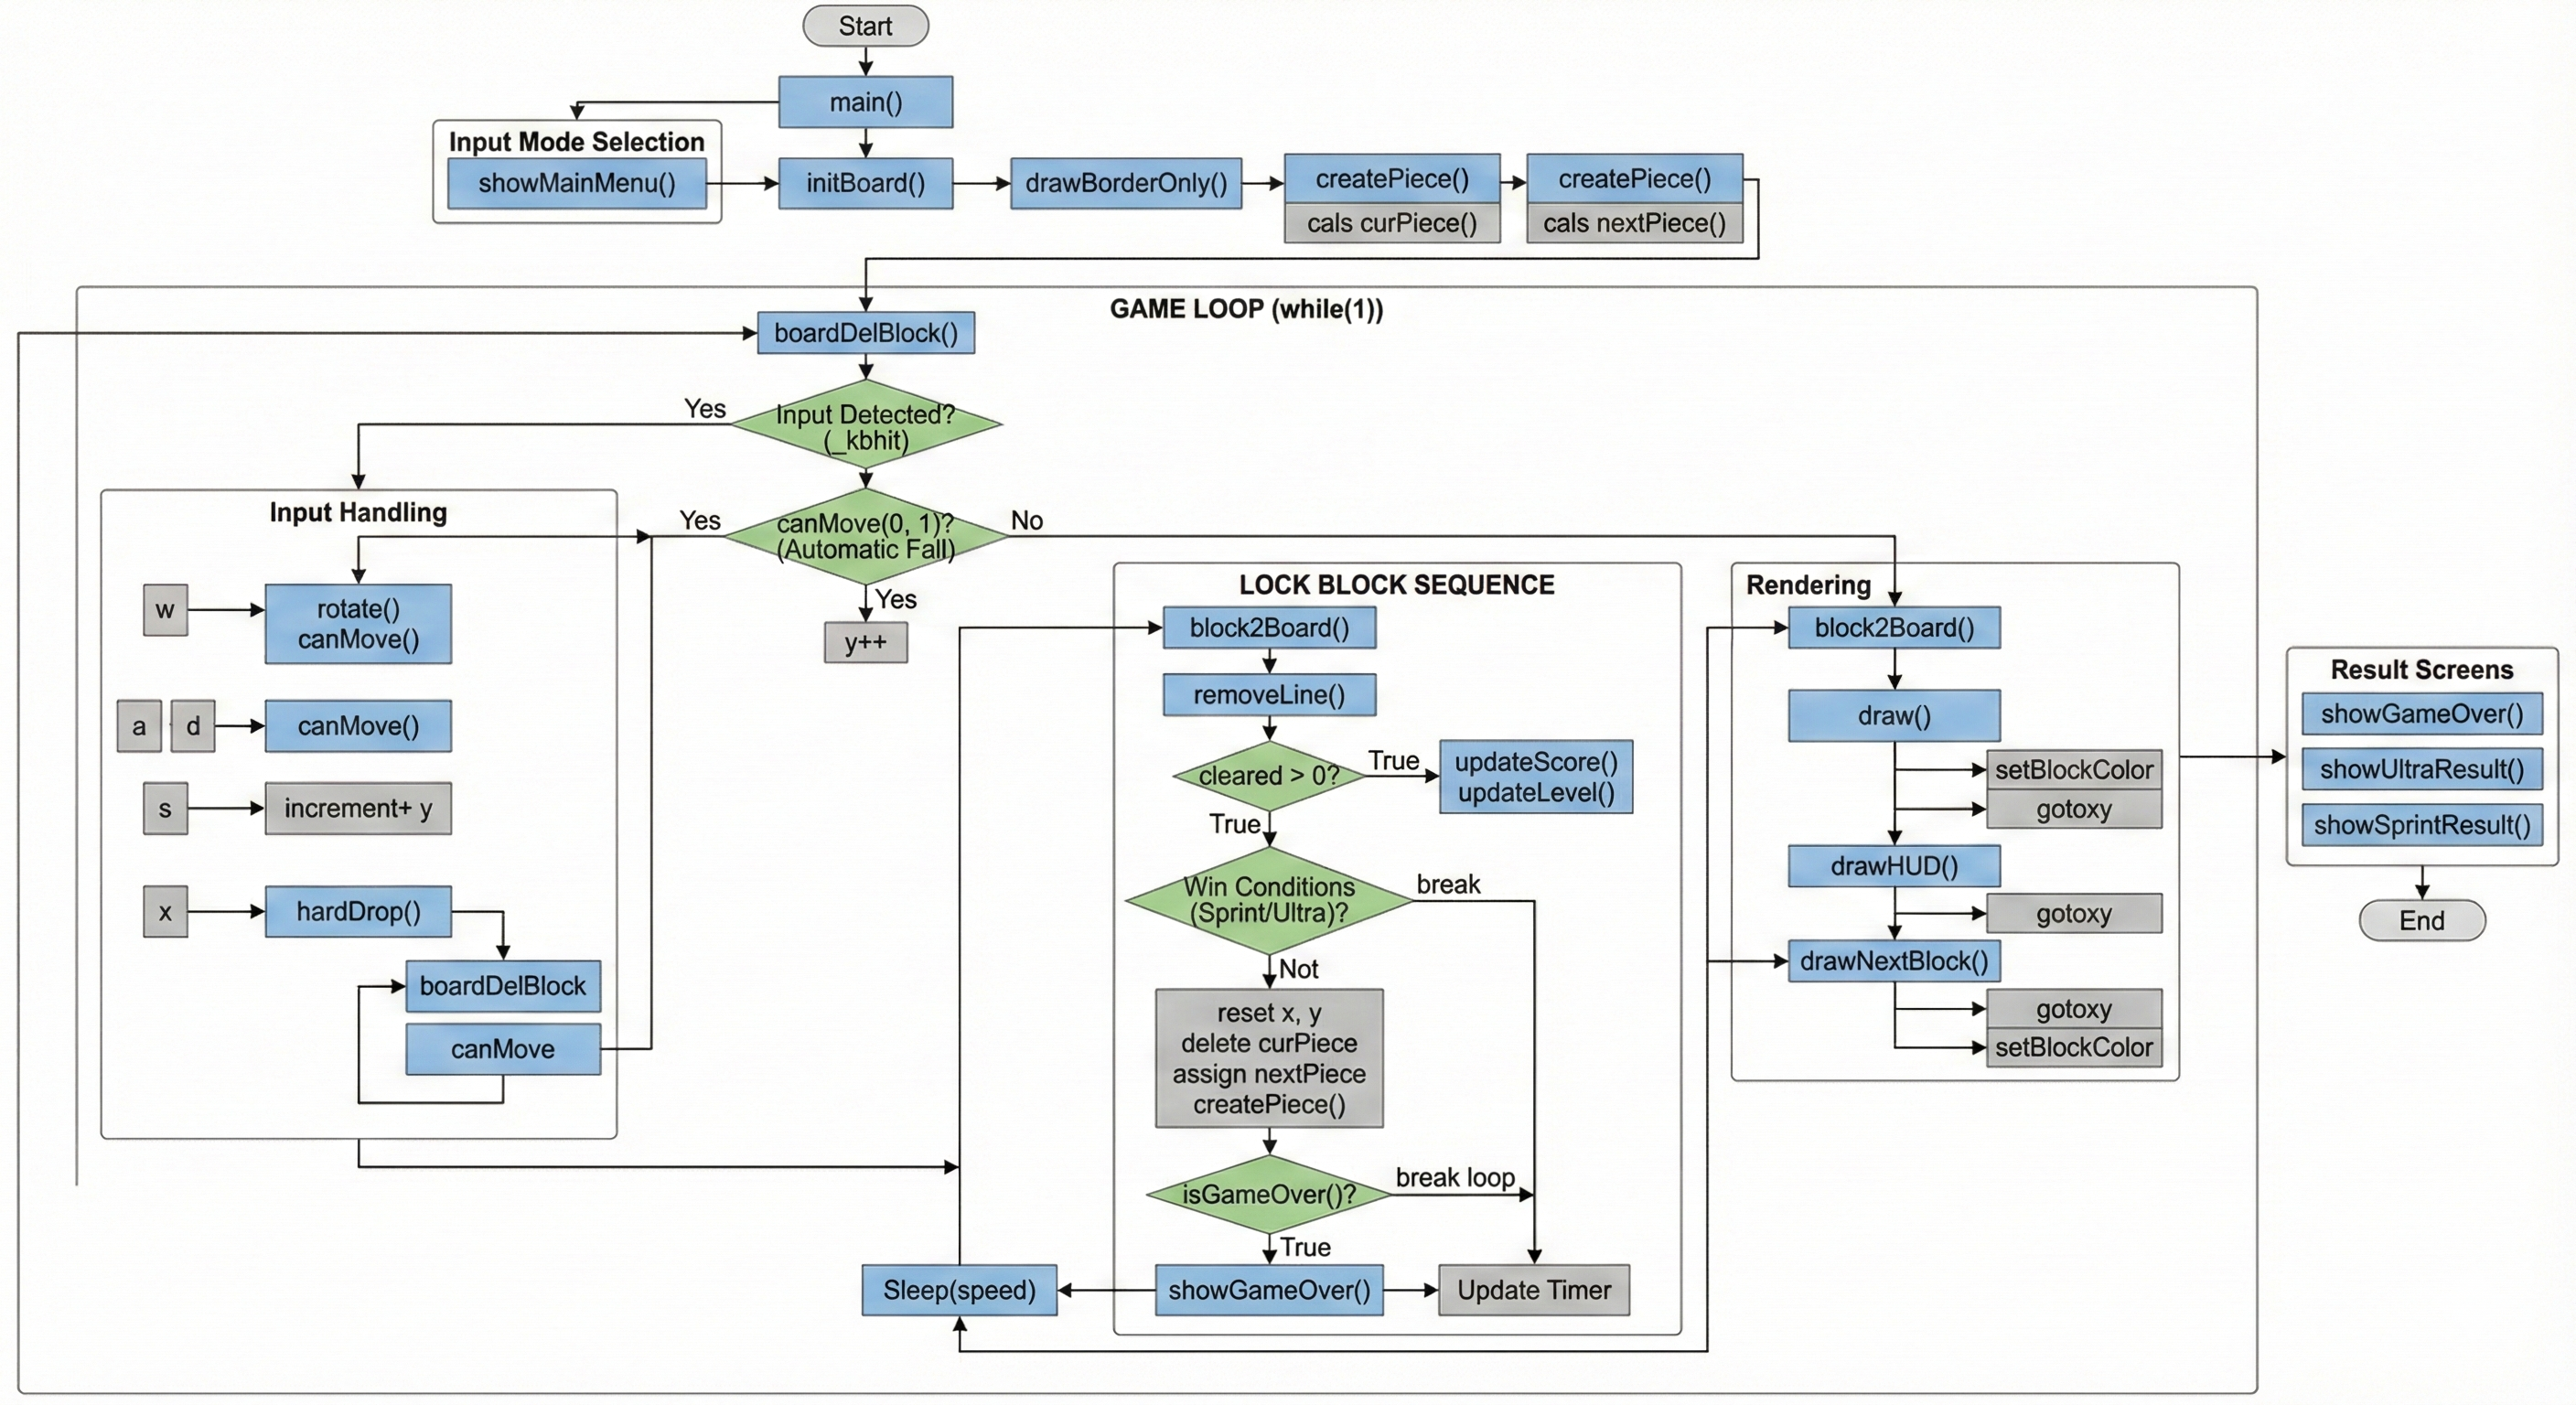
\includegraphics[width=\textwidth]{diagram.png}
    \caption{Sơ đồ thuật toán và luồng xử lý trong game Tetris}
\end{figure}

\subsection{III. Phân tích thuật toán}

\textbf{1. Khai báo thư viện và hằng số}

\noindent
\textless conio.h\textgreater : xử lý bàn phím không chặn (\_kbhit(), \_getch()).\\
\textless windows.h\textgreater : thao tác console (tọa độ, màu, cursor, timer).

\begin{figure}[H]
    \centering
    \includegraphics[width=0.9\textwidth]{thuvien.png}
\end{figure}

\textbf{2. Khai báo kích thước bảng chơi}

\noindent
H: chiều cao bảng\\
W: chiều rộng bảng

\begin{figure}[H]
    \centering
    \includegraphics[width=0.7\textwidth]{kichthuoc.png}
\end{figure}

\textbf{3. Ma trận bảng trò chơi (Board)}

\textbf{Chức năng}

\noindent
Lưu toàn bộ trạng thái game bao gồm : Viền, Ô trống, Các khối đã khóa

\medskip
\textbf{Giá trị trong board}

\noindent
' ' : ô trống\\
'|', '-', '+' : biên\\
'I','O','T','S','Z','J','L' : các block

\medskip
$\rightarrow$ Đây là cấu trúc dữ liệu trung tâm, gần như mọi thuật toán đều đọc/ghi vào board.

\begin{figure}[H]
    \centering
    \includegraphics[width=0.9\textwidth]{matranabang.png}
\end{figure}

\textbf{4. Dữ liệu các khối Tetris (Tetromino)}

\noindent
Lưu 7 khối chuẩn Tetris, mỗi khối là ma trận 4×4

\medskip
\noindent
Ý tưởng thuật toán:\\
Chuẩn hóa kích thước để giúp dễ xoay.\\
Duyệt từng ô để kiểm tra va chạm, gắn vào board và render

\medskip
$\rightarrow$ Đây là nguồn dữ liệu gốc cho mọi khối sinh ra trong game.

\begin{figure}[H]
    \centering
    \includegraphics[width=0.9\textwidth]{dulieukhoi.png}
\end{figure}

\textbf{5. Lớp cơ sở Piece}

\begin{figure}[H]
    \centering
    \includegraphics[width=0.9\textwidth]{loppiece.png}
\end{figure}

\noindent
-Lớp cơ sở Piece đại diện cho một khối đang rơi, có thuộc tính là mảng char shape[4][4] giúp lưu hình dạng hiện tại của khối đang rơi.

\medskip
\noindent
-Đối với phương thức của lớp bao gồm:

\medskip
\noindent
a)Constructor của class piece: Piece(char src[4][4])-> copy dữ liệu từ blocks vào shape, giúp mỗi khối có bản sao riêng, không ảnh hưởng tới nhau

\medskip
\noindent
b)Hàm xoay khối: virtual void rotate();\\
Hàm rotate() được khai báo là virtual để cho phép các lớp con ghi đè hành vi xoay khối, thể hiện tính đa hình trong lập trình hướng đối tượng.

\medskip
\noindent
char temp[4][4] = \{ ' ' \};\\
Tạo ma trận phụ để lưu trạng thái sau khi xoay. Việc dùng ma trận tạm giúp tránh lỗi ghi đè dữ liệu khi xoay trực tiếp trên shape.

\medskip
\noindent
Đối với vòng lặp đầu:

\noindent
temp[j][3 - i] = shape[i][j];\\
Thực hiện phép xoay ma trận 4×4 90 độ theo chiều kim đồng hồ bằng công thức ánh xạ chỉ số. Đây là thuật toán xoay chuẩn cho ma trận vuông.

\medskip
\noindent
Đối với vòng lặp sau:

\noindent
shape[i][j] = temp[i][j];\\
  Sao chép dữ liệu đã xoay từ temp về lại shape, hoàn tất thao tác xoay khối.

\medskip
\noindent
Hàm rotate() chỉ thay đổi hình dạng khối, không kiểm tra va chạm hay biên. Việc kiểm tra hợp lệ sau khi xoay được xử lý ở các hàm khác, giúp chương trình rõ ràng và dễ bảo trì.\\
Riêng khối O, lớp OPiece ghi đè rotate() với thân hàm rỗng vì xoay khối O không làm thay đổi hình dạng, nhưng vẫn đảm bảo tính thống nhất khi gọi hàm thông qua con trỏ Piece*.

\medskip
\noindent
c) Hàm getCell

\noindent
Hàm getCell() dùng để truy cập giá trị tại một ô cụ thể trong ma trận hình dạng shape của khối Tetris.\\
  Tham số i, j lần lượt là chỉ số hàng và cột trong ma trận 4×4 biểu diễn khối.

\noindent
  Hàm trả về ký tự tại vị trí tương ứng:

\noindent
' ' : ô trống\\
'I', 'O', 'T', 'S', 'Z', 'J', 'L' : phần tử của khối.

\textbf{6. Các lớp kế thừa từ Piece}

\begin{figure}[H]
    \centering
    \includegraphics[width=0.9\textwidth]{lopkethuapiece.png}
\end{figure}

\noindent
Các khối I, T, S, Z, J, L: dùng xoay mặc định\\
Riêng O không xoay $\rightarrow$ override rỗng\\
$\rightarrow$ Thể hiện đa hình (polymorphism) rất rõ ràng.

\textbf{7. Hàm tạo khối createPiece()}

\noindent
Hàm createPiece() có nhiệm vụ tạo ra một khối Tetris mới dựa trên chỉ số type và trả về con trỏ kiểu Piece*.

\medskip
\noindent
  Tham số type nhận giá trị từ 0 đến 6, tương ứng với 7 loại khối chuẩn của Tetris.\\
  Cấu trúc switch–case được sử dụng để xác định loại khối cụ thể cần tạo.

\medskip
\noindent
Mỗi nhánh case cấp phát động (new) một đối tượng thuộc lớp con của Piece (IPiece, OPiece, TPiece, …) và truyền dữ liệu hình dạng ban đầu từ mảng blocks.  
Việc trả về con trỏ Piece* cho phép chương trình quản lý các khối khác nhau thông qua một kiểu chung, đồng thời gọi được các hàm ảo như rotate() theo đúng loại khối, thể hiện rõ cơ chế đa hình (polymorphism).  
Hàm này đóng vai trò như một Factory Function, giúp tách biệt quá trình sinh khối khỏi logic game chính, làm cho chương trình dễ mở rộng và bảo trì.

\begin{figure}[H]
    \centering
    \includegraphics[width=0.9\textwidth]{taokhoi.png}
\end{figure}

\textbf{8. Con trỏ khối hiện tại và tiếp theo}

\noindent
Hai con trỏ curPiece và nextPiece được dùng để quản lý vòng đời các khối Tetris trong game.

\medskip
\noindent
  curPiece trỏ tới khối đang rơi trên bảng chơi, là đối tượng trực tiếp chịu tác động từ các thao tác của người chơi như di chuyển, xoay và rơi.\\
  nextPiece trỏ tới khối sẽ xuất hiện tiếp theo, dùng để hiển thị trong khung “Next” và chuẩn bị sẵn cho lần sinh khối kế tiếp.

\begin{figure}[H]
    \centering
    \includegraphics[width=0.9\textwidth]{contro.png}
\end{figure}

\textbf{9. Các biến toàn cục trạng thái game}

\noindent
int x = 6, y = 1;\\
->(x, y): vị trí khối hiện tại trên board

\noindent
int speed, level, linesCleared, score;\\
->Quản lý tốc độ, level, điểm

\noindent
bool isUltraMode, isSprintMode;\\
->Xác định chế độ chơi

\textbf{10. Menu chọn chế độ chơi}

\noindent
Cập nhật giá trị cho biến mode tương ứng với 3 chế độ chơi.

\begin{figure}[H]
    \centering
    \includegraphics[width=0.9\textwidth]{menuchedo.png}
\end{figure}

\subsection{11. Hàm gotoxy()}

\begin{figure}[H]
\centering
\includegraphics[width=0.6\textwidth]{gotoxy.png}
\end{figure}

Hàm gotoxy() dùng để di chuyển con trỏ hiển thị (cursor) của console Windows đến vị trí xác định trước khi in dữ liệu ra màn hình.

\begin{itemize}
  \item Hai tham số x và y lần lượt biểu diễn tọa độ cột và dòng trong cửa sổ console.
  \item Kiểu COORD là cấu trúc của Windows API, dùng để lưu vị trí con trỏ.
  \item Hàm SetConsoleCursorPosition() đặt lại vị trí con trỏ dựa trên tọa độ đã chỉ định.
\end{itemize}

Trong chương trình Tetris, gotoxy() được sử dụng để vẽ lại từng phần màn hình tại vị trí cố định (board, HUD, khối tiếp theo) mà không cần xóa toàn bộ console. Nhờ đó, việc render trở nên mượt hơn, giảm nhấp nháy và tăng hiệu suất hiển thị.  
Hàm này đóng vai trò quan trọng trong cơ chế render theo tọa độ, cho phép game console hoạt động tương tự như một hệ thống đồ họa 2D đơn giản.

\subsection{12. Hàm setBlockColor()}

\begin{figure}[H]
\centering
\includegraphics[width=0.6\textwidth]{setblockcolor.png}
\end{figure}

Hàm setBlockColor() có nhiệm vụ thiết lập màu hiển thị cho từng loại khối Tetris khi vẽ ra màn hình console.

\begin{itemize}
  \item Tham số c là ký tự đại diện cho loại khối (I, O, T, S, Z, J, L).
  \item GetStdHandle(STD\_OUTPUT\_HANDLE) lấy handle của console để thao tác màu sắc.
  \item Cấu trúc switch--case ánh xạ mỗi loại khối với một màu riêng, giúp người chơi dễ phân biệt các khối.
\end{itemize}

Các hằng như FOREGROUND\_RED, FOREGROUND\_GREEN, FOREGROUND\_BLUE và FOREGROUND\_INTENSITY là các cờ của Windows API dùng để pha trộn màu và tăng độ sáng.  
Trong quá trình render, hàm này được gọi trước khi in từng ô của khối, và sau đó màu được reset về mặc định để tránh ảnh hưởng tới các phần khác của giao diện.  
Hàm setBlockColor() giúp cải thiện tính trực quan và trải nghiệm người chơi, đồng thời thể hiện khả năng kiểm soát hiển thị console bằng Windows API.

\subsection{13. Hàm initBoard()}

\begin{figure}[H]
\centering
\includegraphics[width=0.6\textwidth]{initboard.png}
\end{figure}

Hàm initBoard() có nhiệm vụ khởi tạo bảng chơi (board) ngay khi bắt đầu game.

\begin{itemize}
  \item Hai vòng lặp lồng nhau duyệt toàn bộ ma trận board kích thước H $\times$ W.
  \item Các ô góc được gán ký tự '+' để tạo khung.
  \item Các ô viền trên và dưới được gán ký tự '-'.
  \item Các ô viền trái và phải được gán ký tự '|'.
  \item Các ô còn lại bên trong bảng được gán ' ' (ô trống), là khu vực khối Tetris sẽ rơi.
\end{itemize}

Cách khởi tạo này giúp bảng chơi có biên cố định, hỗ trợ các thuật toán kiểm tra va chạm và giới hạn di chuyển khối, đồng thời tạo giao diện rõ ràng cho người chơi.


\subsection{14. Hàm drawBorderOnly()}

\begin{figure}[H]
\centering
\includegraphics[width=0.6\textwidth]{drawboarderonly.png}
\end{figure}

Hàm drawBorderOnly() dùng để vẽ khung bảng chơi ra màn hình console ngay khi bắt đầu game.

\begin{itemize}
  \item gotoxy(0, 0) đưa con trỏ về góc trên bên trái để vẽ bảng tại vị trí cố định.
  \item Hai vòng lặp duyệt toàn bộ ma trận board.
  \item Chỉ các ô nằm ở viền trên, dưới, trái, phải mới được in ký tự tương ứng (+, -, |) đã được khởi tạo trước đó.
  \item Các ô bên trong được in ký tự trống để không vẽ nội dung gameplay tại thời điểm này.
\end{itemize}

Cách vẽ này giúp khung bảng chỉ cần vẽ một lần duy nhất, các lần cập nhật sau chỉ cần vẽ phần bên trong, từ đó giảm nhấp nháy màn hình và tăng hiệu suất render.  
Hàm drawBorderOnly() hỗ trợ cơ chế tách riêng vẽ khung và vẽ nội dung, giúp chương trình rõ ràng và tối ưu hơn.

\subsection{15. Hàm draw()}

\begin{figure}[H]
\centering
\includegraphics[width=0.6\textwidth]{draw.png}
\end{figure}

Hàm draw() chịu trách nhiệm vẽ toàn bộ nội dung gameplay bên trong bảng chơi.

\begin{itemize}
  \item Vòng lặp chỉ duyệt từ 1 đến H-2 và W-2, bỏ qua phần viền vì viền đã được vẽ trước đó.
  \item gotoxy(1, i) đặt con trỏ vào đúng dòng cần vẽ để ghi đè nội dung cũ.
\end{itemize}

Với mỗi ô trong board:
\begin{itemize}
  \item Nếu ký tự khác ' ', đây là một phần của khối Tetris $\rightarrow$ gọi setBlockColor() để đặt màu và in ký tự đặc (char(219)) tạo cảm giác khối liền.
  \item Nếu là ô trống, in khoảng trắng để xóa trạng thái cũ.
\end{itemize}

Sau khi vẽ mỗi ô có màu, màu chữ được reset về mặc định để không ảnh hưởng tới các phần hiển thị khác.  \\

Hàm draw() kết hợp với gotoxy() cho phép render từng frame tại chỗ, giúp game chạy mượt và hạn chế hiện tượng nhấp nháy màn hình.

\subsection{16. Hàm boardDelBlock()}

\begin{figure}[H]
\centering
\includegraphics[width=0.6\textwidth]{boarddeblock.png}
\end{figure}

Hàm boardDelBlock() dùng để xóa tạm thời khối đang rơi khỏi bảng chơi trước khi cập nhật vị trí hoặc trạng thái mới.

\begin{itemize}
  \item Hai vòng lặp duyệt toàn bộ ma trận 4$\times$4 của khối hiện tại.
  \item getCell(i, j) kiểm tra ô nào thực sự thuộc khối (khác ' ').
  \item Với mỗi ô của khối, hàm gán lại vị trí tương ứng trên board thành ' ' để xóa dấu vết cũ.
\end{itemize}

Hàm này được gọi trước khi khối di chuyển, xoay hoặc rơi, nhằm tránh việc khối bị vẽ chồng lên chính nó trong frame tiếp theo.  
boardDelBlock() đóng vai trò quan trọng trong cơ chế cập nhật--vẽ lại (erase \& redraw), giúp quá trình render chính xác và không để lại ``bóng'' của khối cũ trên màn hình.

\subsection{17. Hàm block2Board()}

\begin{figure}[H]
\centering
\includegraphics[width=0.6\textwidth]{block2board.png}
\end{figure}

Hàm block2Board() dùng để ghi khối đang rơi vào bảng chơi (board) tại vị trí hiện tại.

\begin{itemize}
  \item Hai vòng lặp duyệt toàn bộ ma trận 4$\times$4 của curPiece.
  \item getCell(i, j) xác định các ô thực sự thuộc khối (khác ' ').
  \item Với mỗi ô hợp lệ, giá trị tương ứng được gán vào board tại vị trí (y + i, x + j).
\end{itemize}

Hàm này được sử dụng trong hai trường hợp:
\begin{itemize}
  \item Trong quá trình render: để vẽ tạm khối đang rơi lên bảng.
  \item Khi khối chạm đáy hoặc va chạm: để khóa khối vĩnh viễn vào board trước khi sinh khối mới.
\end{itemize}

block2Board() là bước đối lập với boardDelBlock(), cùng nhau tạo nên cơ chế xóa -- vẽ -- cập nhật giúp khối di chuyển mượt mà và chính xác trong mỗi vòng lặp game.

\subsection{18. Thuật toán kiểm tra va chạm canMove()}

\begin{figure}[H]
\centering
\includegraphics[width=0.6\textwidth]{canmove.png}
\end{figure}

Hàm canMove() dùng để kiểm tra một thao tác di chuyển hoặc xoay khối có hợp lệ hay không.

\begin{itemize}
  \item Tham số dx, dy biểu diễn độ dịch chuyển theo trục X và Y so với vị trí hiện tại.
  \item Hai vòng lặp duyệt toàn bộ ma trận 4$\times$4 của khối đang rơi.
  \item Chỉ các ô khác ' ' mới được xét va chạm.
\end{itemize}

Với mỗi ô của khối:
\begin{itemize}
  \item (tx, ty) là tọa độ mới của ô đó sau khi dịch chuyển.
  \item Điều kiện tx < 1 || tx >= W - 1 || ty >= H - 1 đảm bảo khối không vượt biên bảng chơi.
  \item Điều kiện board[ty][tx] != ' ' kiểm tra va chạm với các khối đã được khóa trên board.
\end{itemize}

Nếu bất kỳ ô nào vi phạm điều kiện, hàm trả về false. Ngược lại, nếu tất cả các ô đều hợp lệ, hàm trả về true.  
canMove() là thuật toán nền tảng cho các thao tác di chuyển trái/phải, rơi, hard drop và kiểm tra xoay, đảm bảo tính chính xác và ổn định của gameplay.

\subsection{19. Thuật toán xóa hàng removeLine()}

\begin{figure}[H]
\centering
\includegraphics[width=0.6\textwidth]{removeline.png}
\end{figure}

Hàm removeLine() có nhiệm vụ phát hiện và xóa các hàng đã đầy, đồng thời dồn các hàng phía trên xuống.

\begin{itemize}
  \item Vòng lặp ngoài duyệt các hàng từ dưới lên trên, đúng với quy luật của Tetris.
  \item Vòng lặp trong kiểm tra từng ô trong hàng:
\end{itemize}

\begin{itemize}
  \item Nếu gặp ' ' $\rightarrow$ hàng chưa đầy, dừng kiểm tra.
  \item Nếu duyệt hết mà không gặp ô trống (j == W - 1) $\rightarrow$ hàng đầy.
\end{itemize}

Khi phát hiện hàng đầy:
\begin{itemize}
  \item Biến count tăng để ghi nhận số hàng đã xóa.
  \item Các hàng phía trên được dịch xuống 1 dòng bằng cách sao chép dữ liệu từ trên xuống.
  \item i++ được dùng để kiểm tra lại vị trí hiện tại sau khi dồn hàng, tránh bỏ sót các hàng liên tiếp đầy.
\end{itemize}

Hàm trả về số hàng đã xóa để phục vụ cho việc tính điểm và tăng level.  
removeLine() là thuật toán cốt lõi đảm bảo luật chơi Tetris được thực hiện chính xác.

\subsection{20. Kiểm tra kết thúc game}

\begin{figure}[H]
\centering
\includegraphics[width=0.6\textwidth]{isgameover.png}
\end{figure}

Hàm isGameOver() dùng để kiểm tra điều kiện kết thúc trò chơi ngay sau khi sinh một khối mới.

\begin{itemize}
  \item Hai vòng lặp duyệt toàn bộ ma trận 4$\times$4 của curPiece.
  \item Chỉ các ô thực sự thuộc khối (khác ' ') mới được xét.
  \item (tx, ty) là vị trí của khối mới trên bảng chơi.
\end{itemize}

Nếu tại vị trí sinh khối, trên board đã tồn tại một ô khác ' ' thì điều đó chứng tỏ không còn không gian để đặt khối mới, và trò chơi kết thúc ngay lập tức.  
Hàm trả về true khi xảy ra game over, ngược lại trả về false.  
isGameOver() đảm bảo game kết thúc đúng luật, tránh trường hợp khối mới chồng lên các khối đã khóa trên bảng.

\subsection{21. Hiển thị kết thúc game}

\begin{figure}[H]
\centering
\includegraphics[width=0.6\textwidth]{showgameover.png}
\end{figure}

Xóa màn hình, in ra điểm số, số hàng đã clear, và level, sau đó nhấn phím bất kì để thoát.

\subsection{22. Hard Drop}

\begin{figure}[H]
\centering
\includegraphics[width=0.6\textwidth]{harddrop.png}
\end{figure}

Hàm hardDrop() thực hiện thao tác thả nhanh khối xuống vị trí thấp nhất có thể.

\begin{itemize}
  \item boardDelBlock() xóa tạm thời khối khỏi bảng để tránh va chạm giả với chính nó trong quá trình kiểm tra.
  \item Vòng lặp while (canMove(0, 1)) liên tục kiểm tra khả năng di chuyển xuống dưới.
  \item Nếu còn có thể di chuyển, biến y tăng lên, đẩy khối xuống từng ô cho đến khi chạm đáy hoặc va chạm khối khác.
\end{itemize}

Sau khi vòng lặp kết thúc, khối nằm đúng tại vị trí hợp lệ thấp nhất và sẽ được khóa vào bảng ở vòng lặp gameplay tiếp theo.\\
Hàm hardDrop() giúp tăng tốc độ chơi, đồng thời tận dụng trực tiếp thuật toán canMove() để đảm bảo khối không vượt biên hoặc va chạm.

\subsection{23. Tính điểm updateScore()}

\begin{figure}[H]
\centering
\includegraphics[width=0.6\textwidth]{updatescore.png}
\end{figure}

Hàm updateScore() dùng để tính điểm sau khi xóa hàng.

\begin{itemize}
  \item Tham số lines là số hàng đã được xóa trong một lần.
  \item Cấu trúc switch--case áp dụng quy tắc tính điểm chuẩn của Tetris: xóa càng nhiều hàng cùng lúc thì điểm càng cao.
  \item Biến linesCleared được cập nhật để theo dõi tổng số hàng đã xóa trong suốt ván chơi.
\end{itemize}

Hàm này tách riêng việc tính điểm khỏi gameplay, giúp chương trình rõ ràng và dễ điều chỉnh luật tính điểm.

\subsection{24. Tăng level updateLevel()}

\begin{figure}[H]
\centering
\includegraphics[width=0.6\textwidth]{updatelevel.png}
\end{figure}

Hàm updateLevel() dùng để cập nhật level và tốc độ rơi của khối.

\begin{itemize}
  \item Cứ mỗi 10 hàng được xóa $\rightarrow$ tăng 1 level.
\end{itemize}

Khi level tăng:
\begin{itemize}
  \item Tốc độ rơi (speed) giảm 10\%, làm game khó hơn.
  \item Có giới hạn tốc độ tối đa (speed >= 50) để tránh game quá nhanh.
\end{itemize}

\subsection{25. Hiển thị next block}

\begin{figure}[H]
\centering
\includegraphics[width=0.6\textwidth]{nextblock.png}
\end{figure}

Hàm drawNextBlock() dùng để hiển thị khối tiếp theo (nextPiece) ở khu vực bên phải bảng chơi.

boxX, boxY xác định tọa độ cố định của khung ``Next'' trên console.
\begin{verbatim}
gotoxy(boxX, boxY);
cout << "Next";
\end{verbatim}

In tiêu đề ``Next'' để người chơi biết khối sắp xuất hiện.  
Các vòng lặp tiếp theo vẽ khung chữ nhật bao quanh khối tiếp theo bằng ký tự |, -, +, giúp giao diện rõ ràng.

\begin{verbatim}
for (int i = 0; i < 4; i++) {
    gotoxy(boxX + 1, boxY + 2 + i);
    for (int j = 0; j < 4; j++) {
        char c = nextPiece->getCell(i, j);
\end{verbatim}

Duyệt ma trận 4$\times$4 của nextPiece.

Nếu ô khác ' ' $\rightarrow$ đặt màu bằng setBlockColor() và in ký tự khối.  
Nếu là ô trống $\rightarrow$ in khoảng trắng.

\subsection{26. HUD}

\begin{figure}[H]
\centering
\includegraphics[width=0.6\textwidth]{hud.png}
\end{figure}

Hàm này hiển thị điểm số, số hàng đã xóa và level hiện tại.  
Nếu Ultra Mode $\rightarrow$ hiển thị thời gian còn lại.  

Ngược lại $\rightarrow$ hiển thị thời gian đã chơi.

\subsection{27. Ultra \& Sprint Result}

\begin{figure}[H]
\centering
\includegraphics[width=0.6\textwidth]{ultraandsprint.png}
\end{figure}

Hàm showUltraResult() được gọi khi thời gian chơi đạt giới hạn 120 giây trong chế độ Ultra.  
Hàm thực hiện các chức năng:

\begin{itemize}
  \item Xóa màn hình console để chuyển sang giao diện tổng kết.
  \item Hiển thị các thông số cuối cùng của ván chơi gồm: điểm số, số hàng đã xóa và level đạt được.
  \item Tạm dừng chương trình và chờ người chơi nhấn phím.
\end{itemize}

Chế độ Ultra không phụ thuộc vào trạng thái đầy của bảng chơi mà kết thúc dựa trên thời gian, mục tiêu chính là đạt điểm số cao nhất trong khoảng thời gian cố định.

Hàm showSprintResult() được gọi khi số hàng đã xóa đạt ngưỡng 40 hàng trong chế độ Sprint.  
Chức năng của hàm:

\begin{itemize}
  \item Xóa màn hình và hiển thị giao diện kết quả.
  \item Hiển thị thời gian hoàn thành và tổng số hàng đã xóa.
  \item Dừng chương trình để người chơi xem kết quả.
\end{itemize}

Chế độ Sprint là chế độ đua tốc độ, trong đó điểm số không phải yếu tố đánh giá chính mà thời gian hoàn thành là tiêu chí quan trọng nhất.

\subsection{28. Hàm main()}

\begin{figure}[H]
\centering
\includegraphics[width=0.6\textwidth]{main.png}
\end{figure}

Trong giai đoạn đầu, hàm main() thực hiện:

\begin{itemize}
  \item Khởi tạo bảng chơi bằng initBoard().
  \item Khởi tạo điểm số, level, tốc độ rơi và số hàng đã xóa.
  \item Sinh khối đầu tiên (curPiece) và khối tiếp theo (nextPiece) bằng createPiece().
  \item Lưu thời điểm bắt đầu để tính thời gian chơi cho Sprint và Ultra.
\end{itemize}

Giai đoạn này đảm bảo trò chơi sẵn sàng trước khi vào vòng lặp chính.

\subsection{29. Vòng lặp game chính}

\begin{figure}[H]
\centering
\includegraphics[width=0.6\textwidth]{vonglapchinh.png}
\end{figure}


\begin{figure}[H]
\centering
\includegraphics[width=0.6\textwidth]{vonglapchinh2.png}
\end{figure}

Vòng lặp vô hạn đại diện cho toàn bộ thời gian diễn ra ván chơi.

\subsubsection*{a) Xử lý thời gian và điều kiện kết thúc}

\begin{itemize}
  \item Cập nhật thời gian đã chơi.
  \item Nếu chế độ Ultra và thời gian >= 120 giây $\rightarrow$ kết thúc game và gọi showUltraResult().
  \item Nếu chế độ Sprint và linesCleared >= 40 $\rightarrow$ kết thúc game và gọi showSprintResult().
\end{itemize}

\subsubsection*{b) Xử lý nhập liệu (Input)}

Sử dụng \_kbhit() và \_getch() để đọc phím:

\begin{itemize}
  \item A / D: di chuyển khối sang trái / phải.
  \item W: xoay khối.
  \item S: tăng tốc rơi.
  \item X: hard drop.
  \item ESC: thoát game.
\end{itemize}

Nhập liệu được xử lý theo thời gian thực, không làm gián đoạn vòng lặp.

\subsubsection*{c) Cập nhật logic game}

\begin{itemize}
  \item Kiểm tra khả năng rơi của khối hiện tại.
  \item Nếu không thể rơi $\rightarrow$ khóa khối vào bảng (block2Board()).
  \item Thực hiện xóa hàng (removeLine()).
  \item Cập nhật điểm số (updateScore()).
  \item Cập nhật level và tốc độ (updateLevel()).
  \item Sinh khối mới và kiểm tra điều kiện game over (isGameOver()).
\end{itemize}

Đây là phần xử lý thuật toán cốt lõi của gameplay.

\subsubsection*{d) Vẽ giao diện (Render)}

\begin{figure}[H]
\centering
\includegraphics[width=0.6\textwidth]{vonglapchinh2.png}
\end{figure}

\begin{itemize}
  \item Vẽ bảng chơi và các khối (draw()).
  \item Vẽ thông tin HUD (drawHUD()).
  \item Vẽ khối tiếp theo (drawNextBlock()).
\end{itemize}

Việc tách riêng render giúp game ổn định và dễ mở rộng.

Khi game kết thúc theo từng chế độ hoặc xảy ra game over:
\begin{itemize}
  \item Thoát vòng lặp.
  \item Hiển thị kết quả tương ứng.
  \item Giải phóng bộ nhớ các khối (delete curPiece, delete nextPiece).
\end{itemize}

















\section{4. Đánh giá quá trình làm việc nhóm}

\subsection{I. Mô tả quá trình làm việc nhóm}

Trong quá trình thực hiện đồ án, nhóm chúng em gồm 5 thành viên đã phối hợp làm việc một cách nghiêm túc và có tổ chức. Nhóm có sự phân công nhiệm vụ rõ ràng, các thành viên hỗ trợ lẫn nhau nhằm hoàn thành sản phẩm đúng tiến độ và đáp ứng yêu cầu của học phần. Mặc dù mỗi thành viên có thế mạnh và kỹ năng khác nhau, nhưng toàn nhóm luôn duy trì tinh thần trách nhiệm, hợp tác và chủ động trong công việc.

Ngay từ giai đoạn đầu, nhóm đã thống nhất mục tiêu chung của đồ án, xác định rõ phạm vi thực hiện, yêu cầu về mặt kỹ thuật cũng như hình thức trình bày sản phẩm cuối cùng. Trên cơ sở đó, nhóm tiến hành xây dựng kế hoạch làm việc tổng thể, phân chia các mốc thời gian cụ thể cho từng giai đoạn và thống nhất phương thức phối hợp giữa các thành viên trong suốt quá trình thực hiện.

\subsubsection{1. Phân công nhiệm vụ và tổ chức làm việc}

Việc phân công nhiệm vụ trong nhóm được thực hiện dựa trên năng lực, thế mạnh và mức độ phù hợp của từng thành viên, thay vì phân chia công việc một cách máy móc hoặc ``chia đều'' số lượng nhiệm vụ cho mỗi người. Mỗi thành viên đều có những điểm mạnh riêng, do đó nhóm ưu tiên giao các phần việc phù hợp để phát huy tối đa khả năng cá nhân, đồng thời nâng cao hiệu quả làm việc chung.

Cụ thể, các công việc chính của đồ án được phân chia thành các mảng như: thiết kế và phân tích thuật toán, lập trình các chức năng chính của game, xử lý giao diện hiển thị, kiểm thử chương trình, viết và chỉnh sửa báo cáo, cũng như chuẩn bị nội dung thuyết trình PowerPoint (chi tiết phân công được trình bày tại Mục III của báo cáo).

Ví dụ, các bạn Vinh và Vỹ là những thành viên có kỹ năng lập trình tương đối vững so với các bạn còn lại, nên được giao đảm nhận các phần code quan trọng của chương trình, đồng thời hỗ trợ kiểm tra và góp ý cho code của các thành viên khác. Trong khi đó, bạn Thu Phương có thế mạnh về kỹ năng văn phòng, đặc biệt là các kỹ năng MOS, nên phụ trách chỉnh sửa, căn chỉnh báo cáo, đảm bảo hình thức trình bày đúng chuẩn, đồng thời tham gia xây dựng slide PowerPoint phục vụ cho việc trình bày đồ án.

Tuy nhiên, để đảm bảo tất cả các thành viên đều có cơ hội rèn luyện cả kỹ năng cứng lẫn kỹ năng mềm, nhóm trưởng không chỉ phân công công việc dựa trên sở trường sẵn có mà còn chủ động phân bổ để các thành viên cùng tham gia vào nhiều công đoạn khác nhau của đồ án. Cụ thể, dù không chuyên sâu về lập trình hoặc soạn thảo văn bản, các thành viên vẫn được khuyến khích và giao nhiệm vụ tham gia vào cả hai mảng: vừa lập trình, vừa tham gia viết và chỉnh sửa báo cáo. Việc này nhằm tránh tình trạng một số thành viên chỉ tập trung vào code trong khi các thành viên khác chỉ thực hiện các công việc văn phòng mà không tiếp xúc với phần lập trình của đồ án.

Cách tổ chức này giúp mỗi thành viên không chỉ phát huy được thế mạnh cá nhân mà còn có cơ hội học hỏi thêm các kỹ năng mới, từ đó nâng cao năng lực toàn diện và hiểu rõ hơn về toàn bộ quá trình thực hiện đồ án.

\subsubsection{2. Quy trình làm việc nhóm}

Trong suốt quá trình thực hiện, nhóm áp dụng một quy trình làm việc tương đối rõ ràng, bao gồm các bước sau:

\textbf{Bước 1: Lên ý tưởng và phân tích yêu cầu}

Nhóm cùng nhau thảo luận để thống nhất ý tưởng xây dựng game, xác định gameplay, các chức năng chính cần có và phạm vi của đồ án. Ở giai đoạn này, nhóm tập trung phân tích yêu cầu của học phần và khả năng thực hiện trong khoảng thời gian cho phép.

\textbf{Bước 2: Phân công công việc}

Dựa trên kế hoạch tổng thể, nhóm tiến hành phân chia nhiệm vụ cụ thể cho từng thành viên, đảm bảo công việc được phân bổ hợp lý, tránh chồng chéo và bỏ sót. Các nhiệm vụ được thống nhất rõ ràng về nội dung, thời hạn và trách nhiệm.

\textbf{Bước 3: Phát triển song song}

Các thành viên làm việc độc lập trên từng module hoặc phần việc được giao. Trong quá trình này, các thành viên thường xuyên cập nhật tiến độ và trao đổi khi gặp khó khăn để kịp thời điều chỉnh.

\textbf{Bước 4: Tích hợp và kiểm thử}

Sau khi hoàn thành các phần riêng lẻ, nhóm tiến hành ghép các module lại với nhau, kiểm tra tính tương thích, sửa lỗi phát sinh và tối ưu chương trình. Đây là giai đoạn đòi hỏi sự phối hợp chặt chẽ giữa các thành viên để đảm bảo sản phẩm hoạt động ổn định.

\textbf{Bước 5: Hoàn thiện tài liệu và báo cáo}

Nhóm tiến hành hoàn thiện báo cáo, chỉnh sửa nội dung và hình thức trình bày, chuẩn bị slide PowerPoint và xuất file PDF cho sản phẩm cuối cùng.

\subsubsection{3. Công cụ hỗ trợ làm việc nhóm}

Trong quá trình thực hiện đồ án, nhóm sử dụng nhiều công cụ hỗ trợ để nâng cao hiệu quả làm việc, bao gồm:
\begin{itemize}
    \item Slack: Dùng để trao đổi chuyên môn, phân công công việc, cập nhật tiến độ và thảo luận các vấn đề kỹ thuật;
    \item GitHub: Quản lý mã nguồn, lưu trữ code và các tài liệu LaTeX, hỗ trợ quản lý phiên bản và làm việc nhóm;
    \item Overleaf: Soạn thảo báo cáo bằng LaTeX;
    \item Zalo: Kênh liên lạc nhanh để nhắc nhở và thông báo các vấn đề khẩn;
    \item PowerPoint: Dùng để xây dựng bài thuyết trình sản phẩm đồ án.
\end{itemize}

\subsubsection{4. Những khó khăn gặp phải và cách giải quyết}

\textbf{4.1. Hạn chế của tài khoản Overleaf}

Do tài khoản email trường không hỗ trợ Overleaf Premium, nhóm gặp khó khăn trong việc đồng bộ và chỉnh sửa báo cáo. Để khắc phục, nhóm đã thống nhất giải pháp:
\begin{itemize}
    \item Tạo một repository trên GitHub;
    \item Upload toàn bộ mã nguồn và các file LaTeX lên GitHub;
    \item Một thành viên chịu trách nhiệm upload nội dung lên Overleaf;
    \item Sau khi hoàn thiện, xuất báo cáo dưới dạng PDF để chia sẻ cho các thành viên còn lại.
\end{itemize}

\textbf{4.2. Khó khăn trong việc liên lạc}

Do mỗi thành viên có thời gian biểu khác nhau và kiểm tra Slack ở các khung giờ không đồng đều, thông tin đôi khi không được cập nhật kịp thời. Nhóm đã giải quyết bằng cách:
\begin{itemize}
    \item Lập thêm một nhóm Zalo;
    \item Sử dụng Zalo để nhắc các thành viên kiểm tra Slack khi có thông báo quan trọng;
    \item Phân định rõ Slack dùng cho công việc chính, còn Zalo dùng cho nhắc nhở nhanh.
\end{itemize}

\textbf{4.3. Áp lực tiến độ và tích hợp code}

Việc ghép các phần code do nhiều thành viên thực hiện dễ phát sinh lỗi không tương thích và xung đột mã nguồn. Trong những trường hợp này, nhóm trưởng đóng vai trò kiểm tra, chỉnh sửa và thống nhất phong cách code để đảm bảo chương trình hoạt động ổn định. Một số thời điểm tiến độ giữa các thành viên chưa đồng đều, việc tích hợp mã nguồn phát sinh conflict và cần thêm thời gian để xử lý. Tuy nhiên, các vấn đề này đã được nhóm chủ động khắc phục thông qua việc thống nhất quy ước làm việc và hỗ trợ lẫn nhau.

\subsubsection{5. Đánh giá chung}

Nhìn chung, quá trình làm việc nhóm diễn ra nghiêm túc, có tinh thần trách nhiệm và hợp tác. Nhóm trưởng giữ vai trò điều phối, tổng hợp ý kiến và hỗ trợ các thành viên khi gặp vướng mắc, góp phần đảm bảo tiến độ chung của đồ án.

Thông qua đồ án này, các thành viên không chỉ hoàn thành sản phẩm theo yêu cầu mà còn:
\begin{itemize}
    \item Nâng cao kỹ năng lập trình C/C++;
    \item Hiểu rõ hơn về cấu trúc game và các thuật toán liên quan;
    \item Rèn luyện kỹ năng làm việc nhóm, giao tiếp và quản lý thời gian;
    \item Thành thạo hơn trong việc sử dụng các công cụ hỗ trợ như GitHub, Slack và Overleaf.
\end{itemize}

Đây là một trải nghiệm học tập mang tính thực tiễn cao, giúp các thành viên chuẩn bị tốt hơn cho các đồ án lớn cũng như môi trường làm việc chuyên nghiệp trong tương lai.

\subsection{II. Các kỹ năng thu nhận được}

\subsubsection{1. Kỹ năng cứng (Hard skills)}

Thông qua quá trình thực hiện đồ án, nhóm không chỉ hoàn thành sản phẩm theo yêu cầu mà còn thu nhận được nhiều kỹ năng quan trọng. Trước hết, đồ án giúp các thành viên nâng cao rõ rệt kỹ năng lập trình C/C++. Trong quá trình xây dựng game, nhóm được tiếp cận và áp dụng nhiều kiến thức quan trọng như:
\begin{itemize}
    \item Tổ chức chương trình theo cấu trúc hợp lý;
    \item Sử dụng struct, biến cục bộ và toàn cục;
    \item Thiết kế và hiện thực các hàm xử lý logic game;
    \item Phân tách chức năng để chương trình dễ đọc, dễ bảo trì;
    \item Kiểm tra lỗi và tối ưu code trong quá trình tích hợp.
\end{itemize}

Bên cạnh đó, nhóm cũng hiểu rõ hơn về cấu trúc game và các thuật toán liên quan, bao gồm:
\begin{itemize}
    \item Thuật toán xử lý va chạm;
    \item Thuật toán xoay khối, xóa hàng;
    \item Cách quản lý trạng thái game;
    \item Cách tổ chức vòng lặp chính và cập nhật giao diện theo thời gian thực.
\end{itemize}

\subsubsection{2. Kỹ năng mềm (Soft skills)}

Song song với kỹ năng chuyên môn, đồ án cũng giúp nhóm rèn luyện nhiều kỹ năng mềm quan trọng như làm việc nhóm, giao tiếp, quản lý thời gian và phối hợp tiến độ công việc.

\subsubsection{3. Kỹ năng sử dụng công cụ và phần mềm hỗ trợ}

Thông qua đồ án, nhóm chúng em trở nên thành thạo hơn trong việc sử dụng các công cụ hỗ trợ học tập và làm việc nhóm như GitHub, Slack, Overleaf và các công cụ văn phòng.

\subsection{III. Bảng phân công nhiệm vụ}

\renewcommand{\arraystretch}{1.4}
\begin{table}[H]
\centering
\small
\begin{tabular}{|c|p{3cm}|c|p{2.2cm}|p{7.5cm}|c|}
\hline
\textbf{STT} & \textbf{Họ và tên} & \textbf{MSSV} & \textbf{Vai trò} & \textbf{Công việc thực hiện} & \textbf{Mức độ hoàn thành} \\
\hline

1 & Man Mỹ Phương & 24521414 & Nhóm trưởng &
Lập kế hoạch, tìm và nghiên cứu tài liệu liên quan, lập dàn ý cho game, bài báo cáo, đồ án, hợp đồng nhóm, giới thiệu game.  

Phân công nhiệm vụ cho các thành viên.  

Chỉnh sửa hệ thống điều khiển của game, viết báo cáo các kỹ năng và thuật toán nhóm đã sử dụng; vẽ sơ đồ diagram; phân tích thuật toán: struct Piece, các biến cục bộ, chức năng các hàm đặc biệt (gotoxy, initBoard, drawNextBlock, drawHUD); hiện thực chương trình.  

Viết lời mở đầu, lời chào, lời kết trong phần giới thiệu game.  

Vẽ giao diện LEVEL/score/khối tiếp theo/số hàng đã xóa; xây dựng hàm drawNextBlock(), drawHUD().  

Góp ý và chỉnh sửa bài làm của các thành viên; theo dõi sát sao tiến độ bài làm; tổng hợp và hoàn thiện bài báo cáo.  

Tham gia chỉnh sửa, định dạng Overleaf.  

Đánh giá quá trình làm việc nhóm, tổng kết các kỹ năng mềm và cứng mà nhóm gặt hái được, và mức độ thành thạo trong việc sử dụng các công cụ hỗ trợ trong quá trình làm việc.  

Hỗ trợ làm PowerPoint.
& 100\% \\
\hline

2 & Trần Thu Phương & 24521419 & Thành viên &
Viết giao diện người dùng (UI) và điều khiển trong phần giới thiệu game.  

Viết hàm removeLine(), isGameOver().  

Tham gia làm PowerPoint.
& 100\% \\
\hline

3 & Thành Công Vinh & 24522027 & Thành viên &
Viết hướng dẫn chơi theo tiến trình trong phần giới thiệu game.  

Tăng tốc độ rơi khi removeLine(), updateLevel().  

Xây dựng 3 mode game: Ultra, Sprint, Marathon.  

Code phần hiển thị thông tin game.  

Tô màu cho các khối Tetromino.  

Chỉnh sửa Overleaf.  

Làm PowerPoint.

Thuyết trình
& 100\% \\
\hline

4 & Nguyễn Văn Vỹ & 24522063 & Thành viên &
Viết phần giới thiệu cơ chế gameplay cốt lõi và mẹo nâng cao, các sai lầm cần tránh.  

Xây dựng hàm rotateBlocks(); sửa lại mảng char; updateScore(int lines).  

Code phần hiển thị thông tin game.  

Tham gia làm PowerPoint.

Thuyết trình.
& 100\% \\
\hline

5 & Nguyễn Trần Duy Anh & 205220393 & Thành viên &
Vẽ giao diện viền, block; viết hàm hardDrop().
& 80\% \\
\hline

\end{tabular}
\end{table}



\end{document}
